\documentclass[12pt,a4paper, spanish]{report}
\usepackage[spanish]{babel}
\usepackage[latin1]{inputenc}  % Ambos para solucin de asuntos de idioma
\usepackage[T1]{fontenc}
\usepackage{tocbibind}  % Bibliografa en el indice
\usepackage{titlesec}  % Posibilidad de editar los formatos de chapter y section
%\usepackage{times}  % Fuente de letras
\usepackage{amsmath,amssymb,mathrsfs,mathptmx}  % Matemticas varias
\usepackage{hyperref} % Para escribir URLs



% --- Arreglos varios para la inclusion de imgenes
%\usepackage[pdftex]{graphicx}
%\usepackage[dvips]{graphicx}
\usepackage{graphicx}
\usepackage{epstopdf}
\usepackage{float}
\usepackage{subfigure}
%\usepackage{subfig}
\usepackage{wrapfig}
\usepackage[usenames,dvipsnames]{color}
\DeclareGraphicsExtensions{.png,.jpg,.pdf,.mps,.gif,.bmp, .eps}


	

\usepackage{multirow}
\usepackage{multicol}
\usepackage{tabulary}
\usepackage[table]{xcolor}
\usepackage{color}
\usepackage{listings}
%\usepackage{subfloat}
\usepackage{tikz}

\setcounter{secnumdepth}{3}
\setcounter{tocdepth}{3}


% --- Para las dimensiones de los mrgenes etc
\frenchspacing \addtolength{\hoffset}{-1.5cm}
\addtolength{\textwidth}{3cm} \addtolength{\voffset}{-2.5cm}
\addtolength{\textheight}{4cm}
% --- Para el encabezado
\usepackage{fancyhdr}
\fancyhead[R]{2012}\fancyhead[L]{enCuadro} \fancyfoot[C]{\thepage}
\pagestyle{fancy}

% --- Formato de la etiqueta Chapter
%\newcommand{\bigrule}{\titlerule[0.5mm]}
%\titleformat{\chapter}[display]{\bfseries\Huge}
%{\Large\chaptertitlename\ \Large\thechapter}
%{0mm} {\filleft} [\vspace{0.5mm} \bigrule]

\titleformat{\chapter}[display]
{\normalfont\Large\filcenter}
{\titlerule[1pt]%
\vspace{1pt}%
\titlerule
\vspace{1pc}%
\LARGE\MakeUppercase{\chaptertitlename} \thechapter}
{1pc}
{\titlerule
\vspace{1pc}%
\Huge}

%-------------------------

\begin{document}
% Esto es para que se muestren todas las referencias aunque no se citen:
\nocite{*}

\renewcommand{\tablename}{Tabla}
\renewcommand{\theenumi}{\Roman{enumi}}
\renewcommand{\labelenumi}{[\textbf{\theenumi}]}
\renewcommand{\thefootnote}{\arabic{footnote}}
% --- Modificacin de entornos enumerate
\renewcommand{\theenumi}{\roman{enumi}}
\renewcommand{\labelenumi}{\theenumi)}
% --- Modificacin de entornos enumerate

% --- Para hacer highlights
\newcommand{\highlAmarillo}[1]{\colorbox{yellow}{#1}}
\newcommand{\highlVerde}[1]{\colorbox{green}{#1}}
\newcommand{\highlRojo}[1]{\colorbox{red}{#1}}

%



\chapter{Implementaci�n}
\label{chap: imp}
\section{Introducci�n}
En este cap�tulo se muestra la integraci�n de los conocimientos adquiridos a lo largo del proyecto para poder llevar a cabo la realidad aumentada en una aplicaci�n real. Si bien el objetivo principal del proyecto era la exploraci�n de distintos m�todos y algoritmos, parec�a importante poder poner en pr�ctica todo lo desarrollado en un producto final que pudiera parecerse a un prototipo de aplicaci�n comercial. En particular se desarroll� una aplicaci�n pensando en los cuadros de la planta baja del Museo Nacional de Artes Visuales (MNAV). Entre otros autores, tiene cuadros de Pedro Figari, Juan Manuel Blanes y de Joaqu�n Torres Garc�a, que se eligieron para hacer el prototipo. Se sigui� la l�nea que se plante� desde un inicio que fue la de tener tres partes fundamentales: Navegaci�n, Identificaci�n y Realidad Aumentada. Para eso se incorporaron a la aplicaci�n las siguientes funcionalidades:
 \begin{itemize}
\item Navegaci�n por detecci�n de QRs.
\item Identificaci�n de obras mediante SIFT.
\item Comunicaci�n con un servidor.
\item Navegaci�n por listas de cuadros.
\item Interactividad con modelos.
\item Utilizaci�n de redes sociales.
\end{itemize}
En las pr�ximas secciones se describe m�s en detalle cada uno de estos puntos y su integraci�n a la aplicaci�n final. Tambi�n se describe el flujo de la aplicaci�n y algunas clases implementadas.
\section{Diagrama global de la aplicaci�n}
En la descripci�n de las clases que conforman los bloques principales de la aplicaci�n se hace referencia a conceptos de desarrollo sobre Objective-C, as� como tambi�n a \textit{frameworks} y herramientas utilizadas que fueron explicadas en el cap�tulo \ref{chap: hwysw}. Para la comprensi�n del detalle de la implementaci�n es importante conocer estos conceptos de desarrollo.\\
Para que sea m�s sencilla la comprensi�n de los bloques que componen la aplicaci�n, en la Figura \ref{fig: Diaglobal} se muestra un diagrama esquem�tico de la misma que sirve para visualizar c�mo es su flujo \textit{a nivel de usuario}.\\
\begin{figure}[h!]
\centering
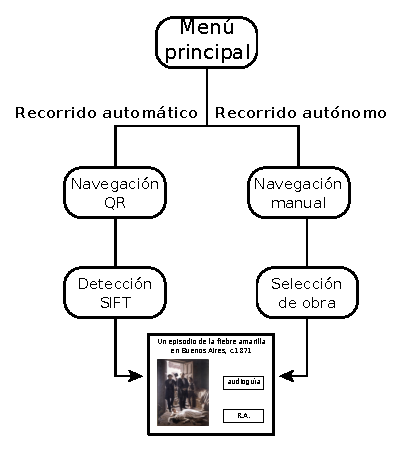
\includegraphics[scale=1.5]{figs_implementacion/implementacion_bloques.eps}
\caption{Diagrama global de la aplicaci�n}
\label{fig: Diaglobal}
\end{figure}
Al comenzar el recorrido, el usuario tiene la opci�n de elegir c�mo recorrer el museo: de manera \textit{aut�noma} o de manera \textit{autom�tica}. En la opci�n aut�noma el usuario es el encargado de elegir dentro de una lista de autores el que m�s le interese, y dentro de la lista de cuadros del autor seleccionado, la obra que desea contemplar en detalle. De esta manera el usuario llega eligiendo opciones al cuadro de inter�s y est� listo para comenzar la interacci�n con la obra, a trav�s de audiogu�as o realidad aumentada. De la otra manera de recorrer el museo, con la opci�n autom�tica, el usuario tiene la opci�n de navegar por el museo leyendo c�digos QR desplegados en las distintas salas o secciones, que sirven para identificar en qu� parte del museo se encuentra el usuario. De esta manera una vez que el usuario lee el QR, la aplicaci�n lo reconoce y despliega una foto del autor y un mensaje que invita al usuario a continuar con el recorrido. Internamente la aplicaci�n guarda la informaci�n en la que est� el usuario y la utiliza en la siguiente etapa: identificaci�n de la de obra. La identificaci�n de la obra se da una vez que el usuario est� frente a la misma y toma una foto de ella que es procesada y en pocos segundos la aplicaci�n responde con la imagen original de la obra y el usuario puede comenzar la interacci�n con la obra, a trav�s de audiogu�as o realidad aumentada. Ver Figura \ref{fig: Diaglobal}\\

De esta manera es que se da el flujo de la aplicaci�n a nivel de usuario, para llegar a un determinado cuadro de inter�s y as� entonces interactuar con �l. Pero este flujo es necesario representarlo en una serie de clases e instancias y con cierta invocaci�n de m�todos que cumplan las reglas de Objective-C con las herramientas existentes de desarrollo que provee Xcode. Para tener una idea de c�mo se mapea el flujo de la aplicaci�n en el lenguaje de desarrollo, en la Figura \ref{fig: story}, se presenta el \textit{Storyboard} de la misma, que muestra la relaci�n entre las distintas clases. Se recuerda al lector que el \textit{Storyboard} es una herramienta de programaci�n gr�fica, que permite generar instancias de clases y v�nculos entre las mismas en forma visual a la vez de ser una representaci�n gr�fica de la interfaz de usuario. A su vez, a la Figura \ref{fig: story} se le agreg� un n�mero identificador en cada \textit{ViewController} para poder referencialos en la medida que sea necesario detallar determinados aspectos de las clases involucradas.\\
\begin{figure}[h!]
\centering
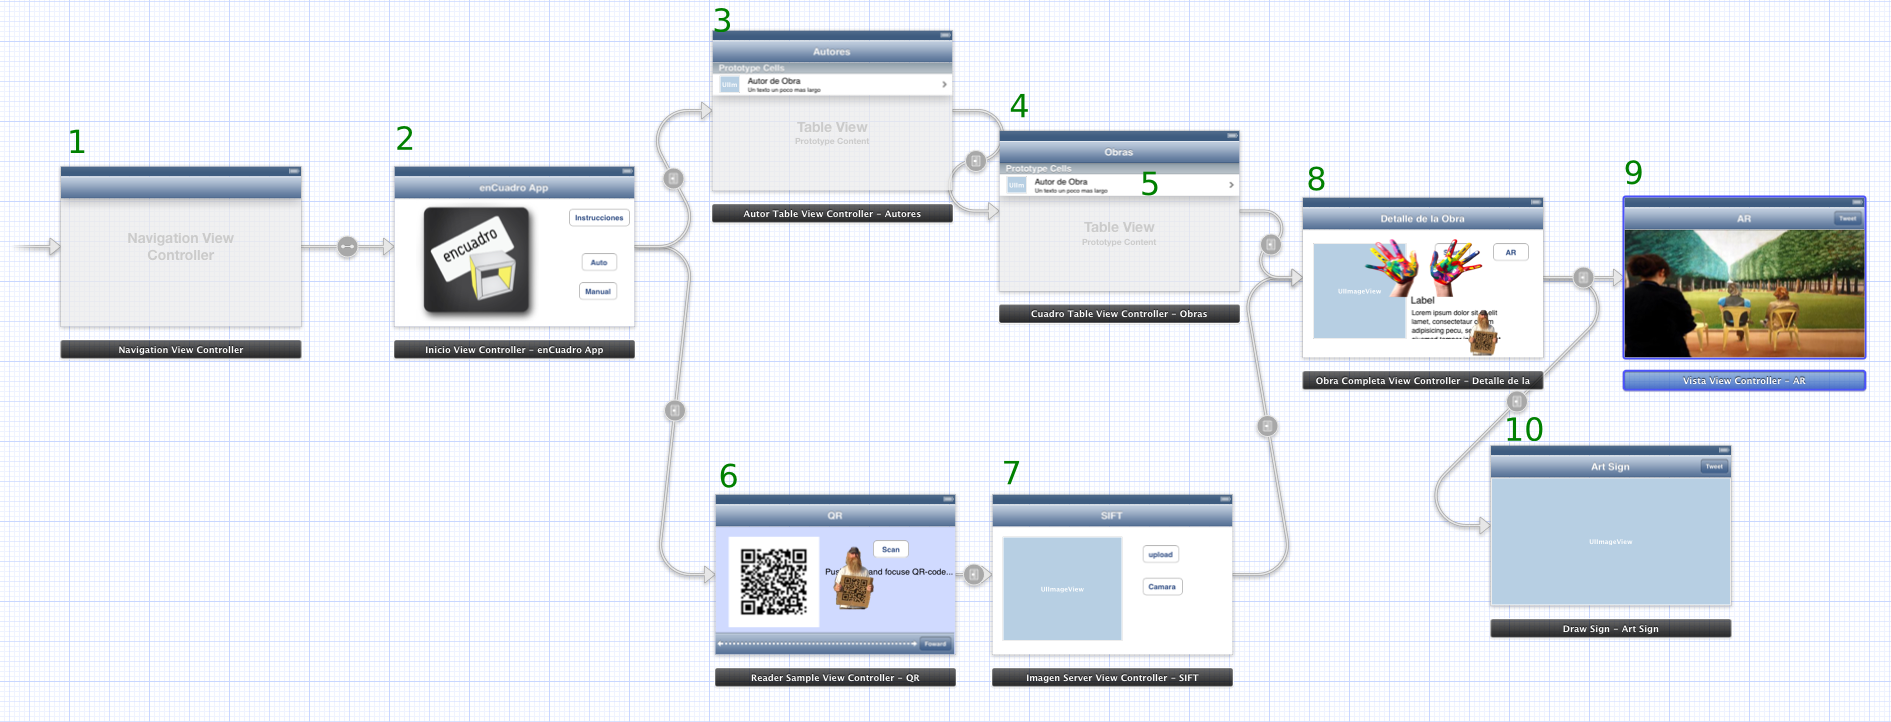
\includegraphics[scale=0.3]{figs_implementacion/Storynum.png}
\caption{\textit{Storyboard} de la aplicaci�n}
\label{fig: story}
\end{figure}
En las pr�ximas subsecciones se explican algunas de las clases implementadas en la aplicaci�n y que adem�s tienen cierta relevancia. Se muestran su rol dentro de la aplicaci�n y sus principales caracter�sticas.
\subsection{NavigationViewController}
Esta clase se ve en la Figura \ref{fig: story}, identificada con el n�mero 1. La aplicaci�n est� embebida dentro de un \textit{UINavigationViewController}. Esto implica que cada uno de los \textit{ViewControllers} que tiene la aplicaci�n es gestionado por esta clase. Es quien se encarga de la presentaci�n y del pasaje de un \textit{ViewController} a otro, creando y destruyendo instancias de cada uno. Est� en esta clase la responsabilidad de manejar las jerarqu�as de los distintos \textit{ViewControllers} as� como de mantener cierta integridad visual utilizando las \textit{Toolbars} ya sea arriba como encabezado o abajo al pie. Las \textit{Toolbars} son botones que se pueden agregar en los extremos de los \textit{ViewControllers} para realizar una funcionalidad espec�fica.\\
El hecho de contar con una jerarqu�a permite entre otras cosas, la posibilidad de hacer un cambio (en la interfaz de usuario por ejemplo), en todos los \textit{ViewControllers}, simplemente afectando a la clase \textit{NavigationViewController} y sin necesidad de cambiar cada uno de ellos por separado. Esto resulta particularmente pr�ctico en aplicaciones con bastantes \textit{ViewControllers} y lo �nico que tiene que hacer el desarrollador es aclarar que ciertos atributos sean manejados por la clase encargada de la navegaci�n dentro de la aplicaci�n. \\
Por otra parte, es deseable tener un criterio com�n para todos los \textit{ViewControllers} en la orientaci�n de la aplicaci�n con respecto a la orientaci�n del dispositivo. Es decir, es posible lograr por ejemplo, que frente a rotaciones del dispositivo, la interfaz de usuario acompa\~ne la rotaci�n y gire tambi�n, o tambi�n es posible permitir que rotaciones del dispositivo en determinado sentido se vean reflejados en una rotaci�n de la interfaz de usuario y otras no. Para esto se definen cuatro posibles posiciones para el dispositivo con ayuda del aceler�metro: \textit{Potrait}, \textit{Upside Down}, \textit{Landscape Left} y \textit{Landscape Right}. Las mismas se pueden ver en la Figura \ref{fig: orientaciones}.

\begin{figure}[h!]
\centering
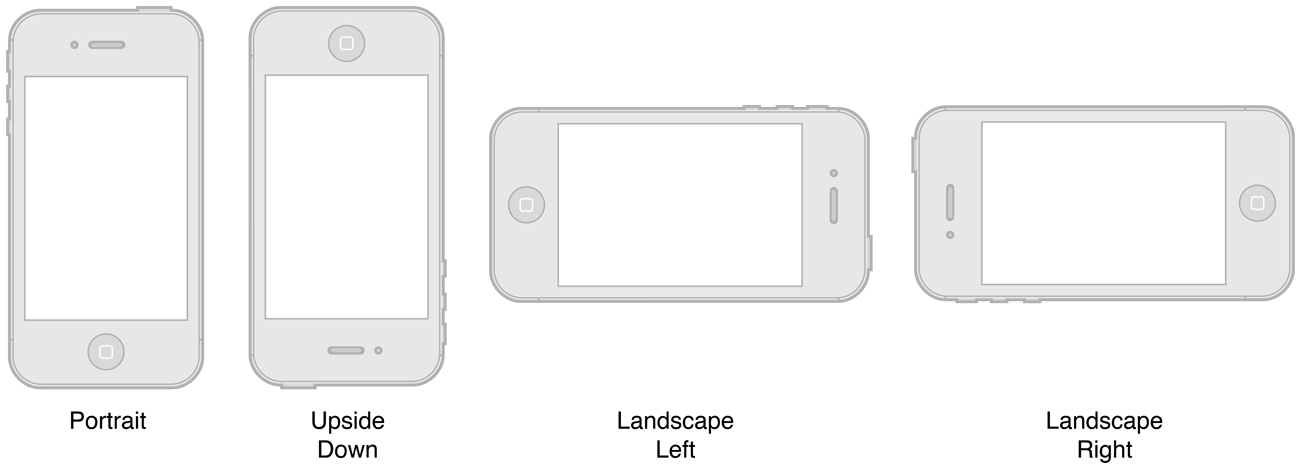
\includegraphics[scale=0.3]{figs_implementacion/orientaciones.png}
\caption{Orientaciones posibles del dispositivo.}
\label{fig: orientaciones}
\end{figure}
%http://developer.apple.com/library/ios/#featuredarticles/ViewControllerPGforiPhoneOS/Introduction/Introduction.html#//apple_ref/doc/uid/TP40007457-CH1-SW1

Para el caso particular de esta aplicaci�n se opt� por reimplementar la clase \textit{UINavigationViewController} bajo el nombre \textit{NavigationViewController} ya que se buscaba tener cierto control sobre las rotaciones de la interfaz de usuario, por lo que se decidi� afectar los m�todos que estuvieran a cargo de las rotaciones de interfaz de usuario. En particular se reimplementaron los m�todos \textit{supportedInterfaceOrientations} y \textit{preferredInterfaceOrientationForPresentation} de la siguiente manera
\begin{verbatim}
-(NSUInteger)supportedInterfaceOrientations
{
    NSLog(@"supportedInterfaceOrientations NAVIGATION");
    return UIInterfaceOrientationMaskLandscapeRight;
}

- (UIInterfaceOrientation)preferredInterfaceOrientationForPresentation
{
    NSLog(@"preferredInterfaceOrientationForPresentation NAVIGATION");
    return UIInterfaceOrientationLandscapeRight;
}
\end{verbatim}
Esto lo que hace es fijar la orientaci�n de la interfaz de usuario a modo \textit{LandscapeRight}. Tambi�n hubiera sido posible lograrlo editando el archivo \textit{Info.plist} que toda aplicaci�n de Xcode tiene, agregando el item \textit{SupportedInterfaceOrientations} y completado las opciones que se desean. Las rotaciones de interfaz de usuario son algo con bastante relevancia en las aplicaciones. En particular se opt� por bloquear las rotaciones de interfaz, dej�ndola fija, para facilitar la reproyecci�n de la realidad aumentada. De no haberlo hecho de esta manera, con cada rotaci�n de la interfaz se tendr�an que intercambiar los ejes de coordenadas en funci�n del sentido de la rotaci�n. Esto es posible de hacer ya que con cada rotaci�n se ejecuta una serie de m�todos en forma autom�tica entre los cuales se encuentra el siguiente:
\begin{verbatim}
- (void) willRotateToInterfaceOrientation:(UIInterfaceOrientation)
toInterfaceOrientation duration:(NSTimeInterval)duration;
\end{verbatim}
Dentro de dicho m�todo ser�a posible hacer el ajuste de coordenadas correspondiente. La serie de m�todos que son ejecutados al haber un evento del tipo rotaci�n es algo que ha sufrido cambios recientes con la actualizaci�n de \textit{software} a iOS 6. 
\subsection{InicioViewController}
Este \textit{ViewController} es la pantalla de inicio  de la aplicaci�n, identificado con el n�mero 2 en la Figura \ref{fig: story}. En la misma hay un bot�n que al ser presionado comienza un audio con instrucciones y una presentaci�n sobre c�mo es el recorrido y las funcionalidades con las que cuenta la aplicaci�n. Tambi�n hay dos botones m�s que dan al usuario la opci�n de elegir la forma de recorrer el museo: aut�noma o autom�tica. El bot�n de recorrido autom�tico instancia al \textit{ReaderSampleViewController} y el de recorrido aut�nomo instancia al \textit{AutorTableViewController}.

\subsection{UITableViewControllers}
Para el recorrido manual, el usuario es el encargado de seleccionar el autor, luego las obras disponibles del autor seleccionado y luego se muestra un detalle de la obra seleccionada por el usuario presentando una instancia del \textit{ViewController} llamado \textit{ObraCompletaViewController}. Este recorrido que parece bastante intuitivo aparece en muchas aplicaciones de iOS en las que existen listas de datos. Un ejemplo son las aplicaciones que gestionan contenido musical que est� ordenado en base a autores, dentro de los mismos, sus discos y dentro de los discos sus canciones. Como navegar en listas de datos es algo bastante frecuente, Xcode ya tiene implementada una clase llamada \textit{UITableViewController}. En la Figura \ref{fig: tablas} se puede ver un ejemplo con varios tipos de tablas que organizan la informaci�n. Como se puede ver la tabla es una forma sencilla de organizar la informaci�n en la que existe una sola columna y muchas filas, llamadas celdas. Tambi�n pueden existir secciones, con un encabezado y pie de secci�n.
\begin{figure}[h!]
\centering
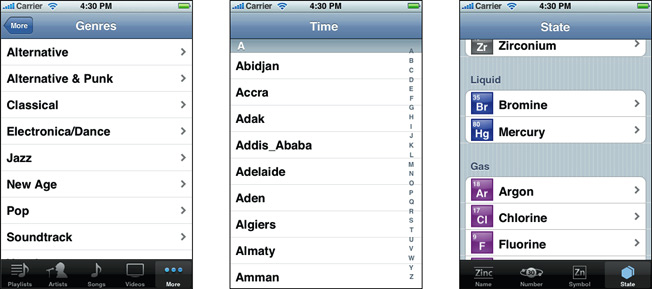
\includegraphics[scale=0.5]{figs_implementacion/types_of_table_views}
\caption{Ejemplos de TableViewControllers con distintos tipos de tablas.}
\label{fig: tablas}
\end{figure}
%http://developer.apple.com/library/ios/#documentation/UserExperience/Conceptual/TableView_iPhone/AboutTableViewsiPhone/AboutTableViewsiPhone.html#//apple_ref/doc/uid/TP40007451-CH1-SW1
Volviendo a la aplicaci�n lo que se hizo entonces fue crear varias clases que heredan de \textit{UITableViewController} y manejar los contenidos de manera jer�rquica. A continuaci�n siguen dos clases que se resolvieron de esta manera.
	\subsubsection{AutorTableViewController}
	Esta clase (identificada con el n�mero 3 en la Figura \ref{fig: story}) hereda de \textit{UITableViewController} y cumple la funci�n de almacenar la lista de autores disponibles dentro del museo que a los efectos del prototipo como se dijo son: Figari, Blanes y Torres Garc�a. En lo que sigue se explican algunos detalles importantes que se tuvieron que comprender para poder organizar la informaci�n en tablas de datos (lo cual tambi�n aplica para la clase \textit{CuadroTableViewController} que se describe en la siguiente subsecci�n).\\
Uno de los m�todos implementados por esta clase es el siguiente:
	\begin{verbatim}
	- (NSInteger)numberOfSectionsInTableView:(UITableView *)tableView
	\end{verbatim}
que por defecto retorna un \textit{0}. El mismo indica la cantidad de secciones con las que cuenta una tabla. Para que tenga sentido y al instanciarse la clase se vea algo de contenido tiene que retornar algo distinto de \textit{0}. Otro m�todo importante es:
	\begin{verbatim}
	- (NSInteger)tableView:(UITableView *)tableView numberOfRowsInSection:
	(NSInteger)section
	\end{verbatim}
	
	El mismo es el encargado de devolver un n�mero con la cantidad de filas con las que cuenta la secci�n de la tabla. En esta implementaci�n se devuelve la cantidad de autores.\\ Un tercer m�todo, de mayor importancia, es el siguiente:
	\begin{verbatim}
	- (UITableViewCell *)tableView:(UITableView *)tableView cellForRowAtIndexPath:
	(NSIndexPath *)indexPath
	\end{verbatim}
	
	El mismo es el encargado de devolver una \textit{UITableViewCell} que es la que se despliega. Es en este m�todo que se configura el formato de la celda. Para el caso de la aplicaci�n se resolvi� generar una clase que hereda de \textit{UITableViewCell} que se llama \textit{CuadroTableViewCell} y que tiene ciertas caracter�sticas como una imagen, autor y obra que son mostradas en la celda. En este m�todo se asocian las caracter�sticas mencionadas de la celda en funci�n del n�mero de fila. Esta clase implementa un m�todo \textit{prepareForSegue} que le asigna un valor a la variable \textit{opcionAutor} en funci�n del autor seleccionado. Esto permite luego en la clase \textit{CuadroTableViewController} desplegar distintas listas de cuadros en funci�n del autor seleccionado.
	\subsubsection{CuadroTableViewController}
	Esta clase (identificada con el n�mero 4 en la Figura \ref{fig: story}) es muy similar a la clase \textit{AutorTableViewController} reci�n descripta pero que difiere simplemente en su contenido. Los conceptos utilizados y m�todos implementados son b�sicamente los mismos pero su contenido es un listado de obras en lugar de autores. Una especificaci�n extra es que al instanciarse la clase se completa una lista de cuadros diferente en funci�n del autor seleccionado. As� como en la clase \textit{AutorTableViewController} en esta tambi�n se implementa el m�todo \textit{prepareForSegue} para poder completar los datos de la instancia de la clase con la que se est� conectando, con los datos de la obra seleccionada (autor, obra, imagen, descripci�n, audio, ARid). El ARid es un identificador de realidad aumentada que asocia una realidad aumentada a cada cuadro.  
	\subsubsection{CuadroTableViewCell}
	Esta es una clase sencilla que hereda de la clase \textit{UITableViewCell} (identificada con el n�mero 5 en la Figura \ref{fig: story}) y simplemente tiene tres  atributos asociados a nivel de interfaz de usuario: una imagen, un nombre de autor y un nombre de obra para cada celda de la tabla que se despliega.\\
\begin{figure}[h!]
\centering
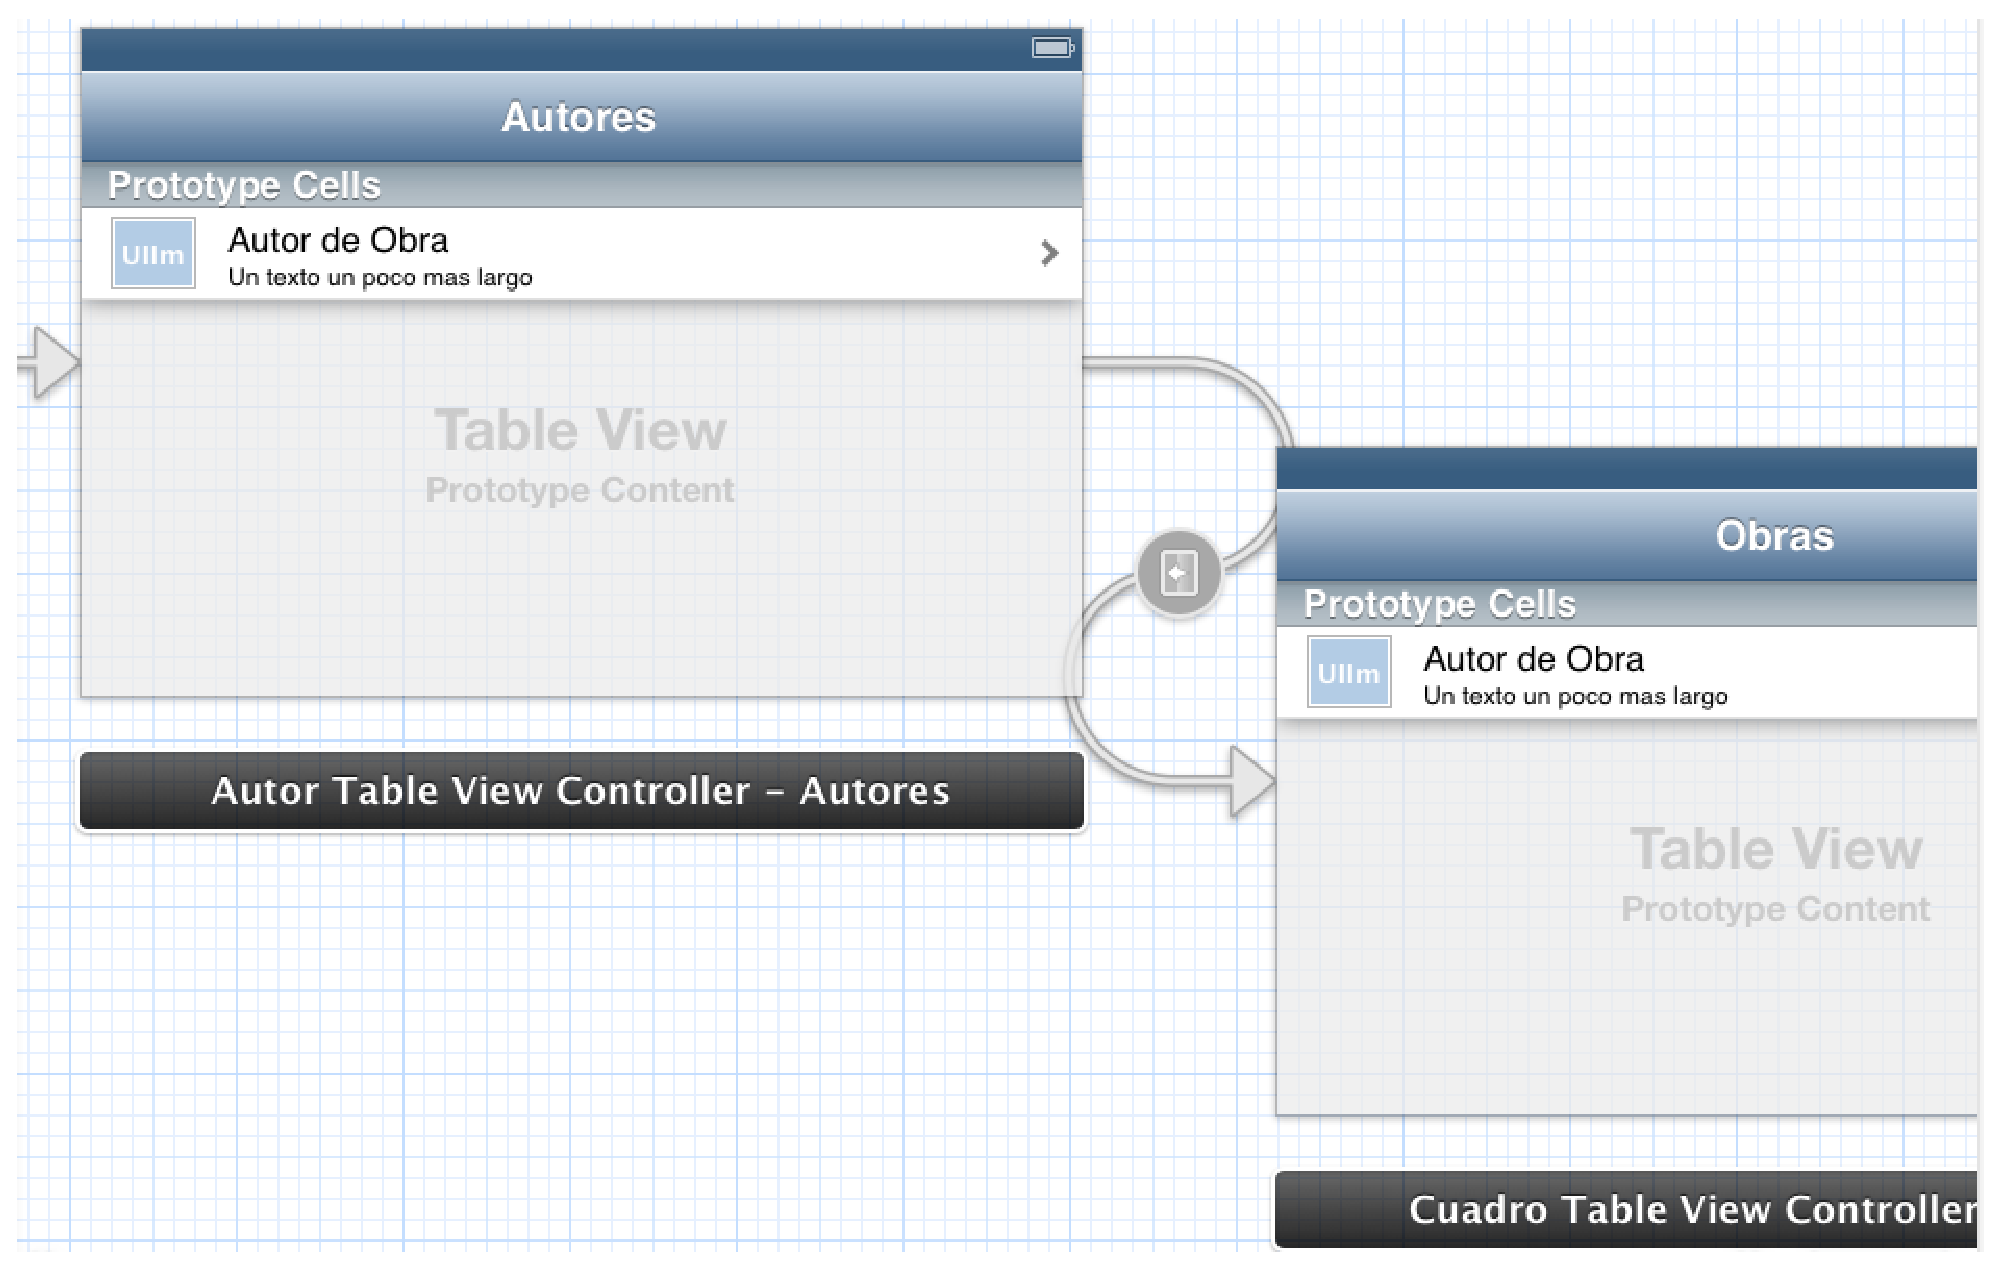
\includegraphics[scale=0.4]{figs_implementacion/AutorYCuadroTable.eps}
\caption{Autor y Cuadro TableViewControllers}
%\label{fig: implementacion_1}
\end{figure}

\subsection{ReaderSampleViewController}
Este \textit{ViewController} (identificado con el n�mero 6 en la Figura \ref{fig: story}) es el encargado de hacer la lectura de los c�digos QR y de invocar los m�todos necesarios para realizar la b�squeda de la zona del museo en la que se encuentra el usuario. Esto es, existe un c�digo QR asociado a cada autor (Blanes, Figari y Torres Garc�a) y en base al c�digo QR le�do se despliega un texto y una imagen asociados al mismo. El funcionamiento de la decodificaci�n se explica un poco m�s en detalle en la secci�n \ref{sec: QR}.

\subsection{ImagenServerViewController}
\label{sec: imagenServer}
Este \textit{ViewController} (identificado con el n�mero 7 en la Figura \ref{fig: story}) es el encargado de la comunicaci�n con el servidor. Al instanciarse esta clase, tambi�n se instancia la clase \textit{UIImagePickerController}, encargada de implementar una captura de imagen. Una vez que se toma una fotograf�a a la obra, la misma se muestra en una \textit{UIImageView} y existen dos botones: uno de ellos simplemente dispara una nueva instancia del \textit{UIImagePickerController} dando la opci�n de volver a tomar la fotograf�a y el otro bot�n inicia la comunicaci�n con el servidor. Ver Figura \ref{fig: imagenServer}.\\
\begin{figure}[h!]
\centering
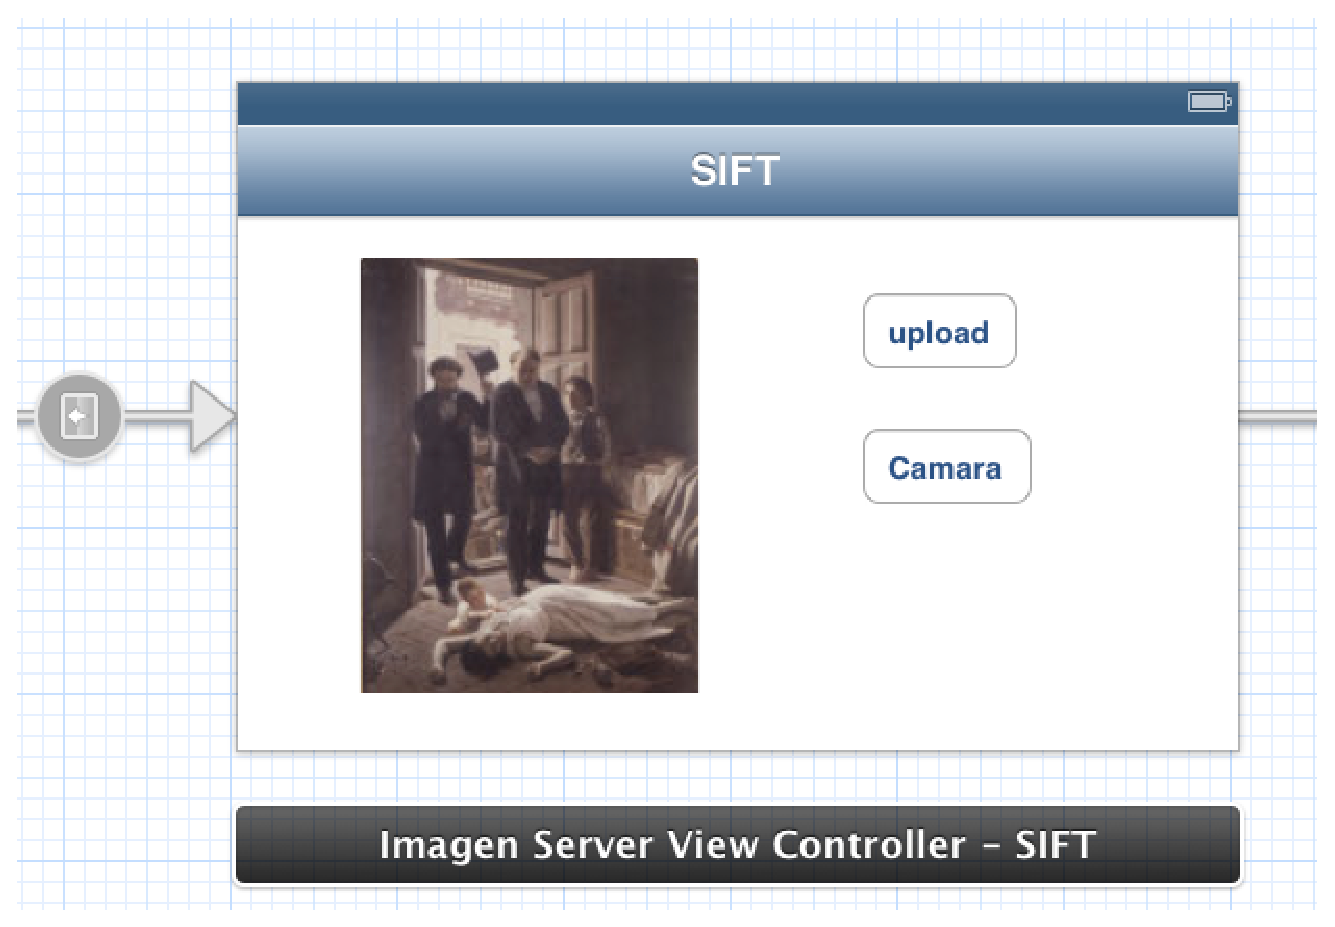
\includegraphics[scale=0.4]{figs_implementacion/imagenServer.eps}
\caption{Ejemplo de captura para reconocimiento SIFT}
\label{fig: imagenServer}
\end{figure}

El bot�n encargado de la comunicaci�n con el servidor, bot�n de \textit{upload}, es un \textit{segue} hacia el \textit{ObraCompletaViewController}. Dentro del m�todo \textit{prepareForSegue}, encargado de preparar todo previo a la invocaci�n de \textit{ObraCompletaViewController} se invoca el m�todo \textit{uploadImage}. Este m�todo genera un mensaje HTTP del tipo POST y se lo env�a a la IP del servidor. En el cuerpo del mensaje se adjunta la foto tomada previamente y se le agrega una variable llamada \textit{room}. Esta variable es completada previamente en el \textit{ReaderSampleViewController} en base al QR detectado, dando informaci�n respecto de en qu� sala/regi�n del museo se encuentra el usuario (sala Figari, sala Blanes o sala Torres Garc�a). Esta variable lo que permite es tener un identificador para poder realizar la b�squeda de la imagen tomada en una base de datos m�s peque\~na, que contenga solamente los cuadros de la regi�n del museo en cuesti�n. En caso que el usuario se haya salteado la detecci�n QR y haya seleccionado directamente la opci�n de tomar una fotograf�a a la obra para comenzar la comunicaci�n con el servidor, entonces la variable \textit{room} estar� vac�a y la b�squeda de la obra se realiza en toda la base de datos del museo. El gran valor agregado de la detecci\'on QR es la velocidad con la que el servidor devuelve informaci\'on respecto de a qu\'e obra se fotografi\'o. Para la b\'usqueda con detecci\'on QR, los tiempos son claramente mejores (del orden de 3s en una LAN), mientras que cuando el usuario se ahorra este paso, los tiempos aumentan al doble (del orden de 6s en una LAN).\\

Luego de establecida la conexi�n y enviada la consulta POST, el servidor responde con otra variable llamada \textit{returnString}. Esta variable contiene un identificador de obra que indica qu� obra fue fotografiada. Esto se logra mediante un archivo \textit{upload.php} en el servidor que recibe la imagen y le ejecuta un algoritmo de detecci�n de caracter�sticas llamado SIFT, que le retorna al PHP el identificador en cuesti�n. Detalles sobre el algoritmo SIFT se pueden ver m�s adelante en la secci�n \ref{sec: sift}. El archivo \textit{upload.php} entrega esta informaci\'on a la aplicaci\'on. La variable \textit{returnString} es recibida por la aplicaci�n con cierta nomenclatura en particular, que sigue la l�gica Autor-N�mero, por ejemplo ``Figari3'' se corresponde con la obra n�mero 3 de la base de datos del autor Figari. Con este identificador de obra, la aplicaci�n le pide al servidor cierta informaci�n de inter�s acerca de la misma, como por ejemplo el nombre completo de la obra, el nombre de su autor y una breve descripci�n. El servidor cuenta con varias carpetas a las que la aplicaci�n accede remotamente:
\begin{itemize}
\item[(1)] \textbf{autor:} contiene el nombre del autor de cada obra. 
\item[(2)] \textbf{obra:} contiene el nombre completo de cada obra.
\item[(3)] \textbf{texto:} contiene una breve descripci�n de cada obra.
\item[(4)] \textbf{imagen:} contiene una imagen de cada obra.
\item[(5)] \textbf{audio:} contiene una audiogu�a asociada a cada obra.
\end{itemize}

Esta informaci�n solicitada es alojada en variables que son mostradas (imagenes, texto) y reproducidas (audio) en el siguiente \textit{ViewController}, el \textit{ObraCompletaViewController}. Ver Figura \ref{fig: obraCompleta}.

\subsection{ObraCompletaViewController}
Este \textit{ViewController} (identificado con el n�mero 8 en la Figura \ref{fig: story}) simplemente es la presentaci�n de la obra en la que se muestra una imagen del cuadro, t�tulo, autor, descripci�n y distintas opciones para interactuar con el mismo. Tiene dos botones y una animaci�n que funciona como bot�n. Ver Figura \ref{fig: obraCompleta}. El primero de los botones dispara una audiogu�a relacionada con la obra que el usuario est� contemplando. El otro bot�n conecta con el \textit{VistaViewController}, encargado de mostrar la realidad aumentada, explicado en la secci�n \ref{sec: vista}. La animaci�n que aparece funciona como \textit{segue} hacia otro \textit{ViewController}, llamado \textit{DrawSign} que se explica m�s adelante en la secci�n \ref{sec: drawsign}.\\
\begin{figure}[h!]
\centering
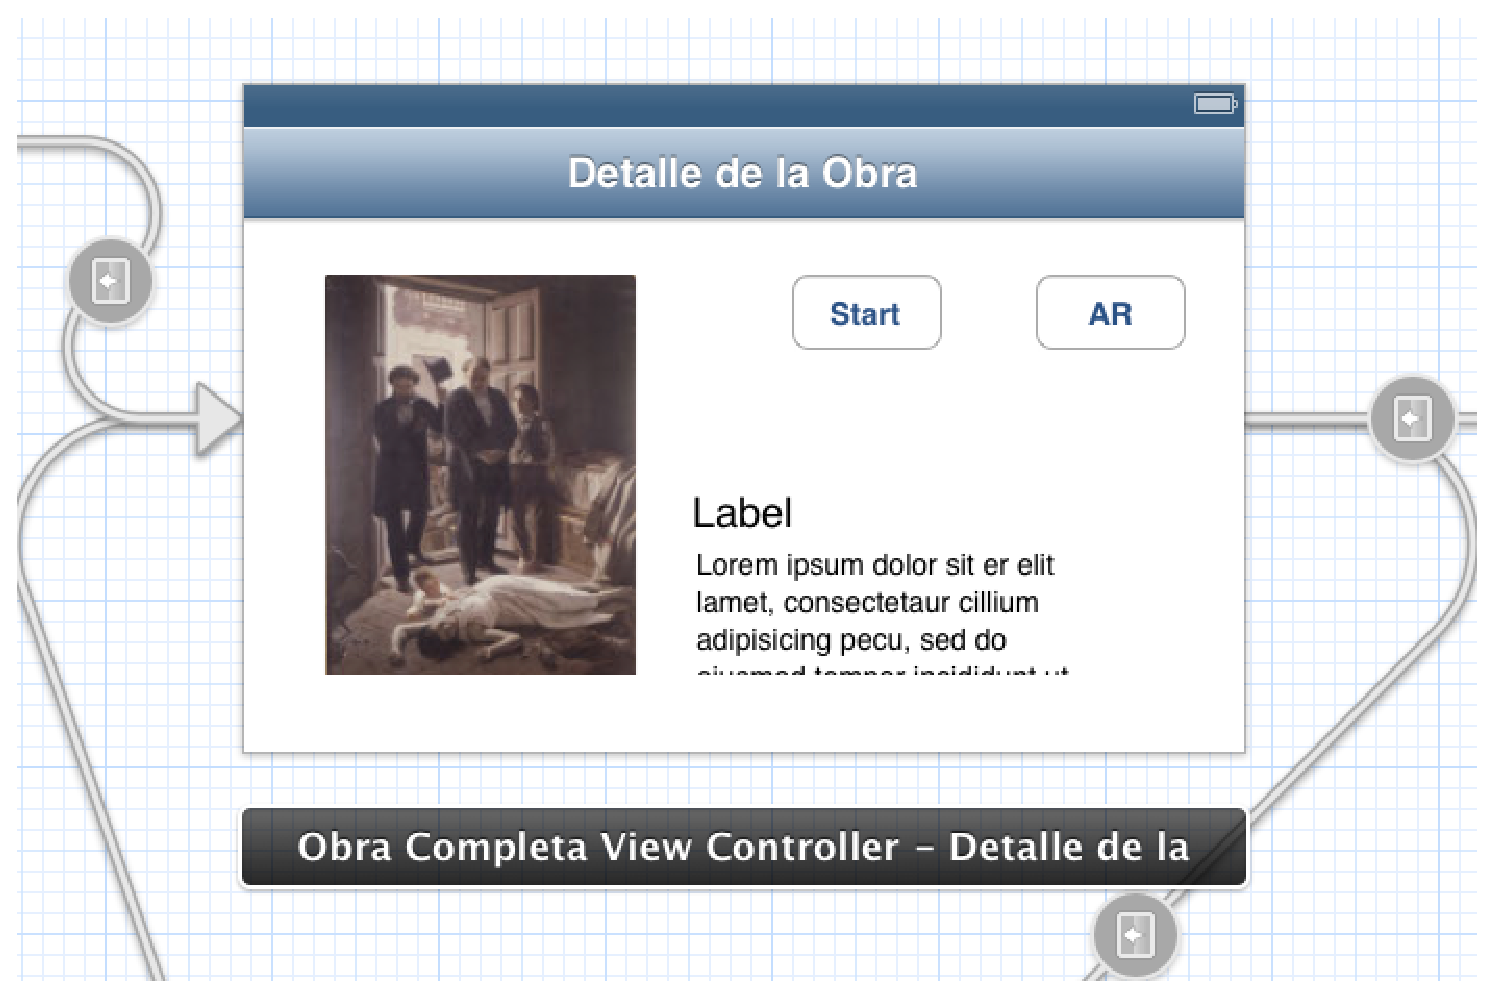
\includegraphics[scale=0.4]{figs_implementacion/ObraCompleta.eps}
\caption{Pantalla con la obra completa}
\label{fig: obraCompleta}
\end{figure}

\subsection{VistaViewController}
\label{sec: vista}
Este \textit{ViewController} (identificado con el n�mero 9 en la Figura \ref{fig: story}) es el encargado de mostrar la realidad aumentada. Esta clase, al ser instanciada ejecuta el siguiente m�todo:
\begin{verbatim}
- (void)viewWillAppear:(BOOL)animated
{
    NSLog(@"VIEW WILL APPEAR VISTA");
    [super viewWillAppear:animated];
   
    [self hacerRender];
     
}
\end{verbatim}
Este m�todo se ejecuta justo antes de que el controlador despliegue el contenido de la pantalla, y como se ve, invoca al m�todo hom�nimo de la clase superior y luego al m�todo \textit{hacerRender}, encargado de mostrar efectivamente la realidad aumentada. Antes de explicar los detalles de \textit{hacerRender} se comentan algunos detalles generales de las aplicaciones iOS.\\

Como en cualquier programa, en las aplicaciones de Xcode, lo que se ejecuta al comenzar es el \textit{main}. En este tipo de aplicaciones en particular, el main crea una instancia de la clase \textit{appDelegate} (delegado de la aplicaci�n). A su vez, al instanciarse al \textit{appDelegate} se ejecuta el m�todo \textit{applicationDidFinishLaunching}. En este m�todo, t�picamente el c�digo por defecto est� vac�o, pero cuando se trabaja con ISGL3D, este m�todo crea un objeto de la clase \textit{Isgl3dViewController} que hereda de \textit{UIViewController}. Es sobre la instancia de \textit{Isgl3dViewController} que se despliegan los \textit{renders}. Aclarados estos puntos se pasa ahora a explicar lo que se hace en el m�todo \textit{hacerRender}. A continuaci�n se muestran algunas de las partes m�s importantes del m�todo:
\begin{verbatim}
app0100AppDelegate *appDelegate = (app0100AppDelegate *)[[UIApplication 
sharedApplication] delegate];
self.viewController=(Isgl3dViewController*)appDelegate.viewController;
\end{verbatim}


Con lo anterior lo que se hace es generar una instancia de la clase \textit{app0100AppDelegate} que es puntero al \textit{appDelegate} de la aplicaci�n. Luego, en la segunda l�nea se le asigna a la propiedad de la clase \textit{VistaViewController} llamada \textit{viewController} (que es de tipo \textit{Isgl3dViewController}) la propiedad de igual nombre pero del \textit{appDelegate} de la aplicaci�n (que fue instanciada en el m�todo \textit{applicationDidFinishLaunching}). Luego se agregan las \textit{views} \textit{viewController.view} y \textit{viewController.videoView} con valor de transparencia \textit{alpha} nulo y se inicia una animaci�n generando un efecto de \textit{fade out} de la imagen y \textit{fade in} del \textit{render}. Este tipo de animaciones son sencillas de ejecutar con el \textit{framework} Core Animation y permiten agregar efectos interesantes a cualquier \textit{UIView}. 

\subsection{DrawSign}
\label{sec: drawsign}
Esta clase (identificada con el n�mero 10 en la Figura \ref{fig: story}) hereda de \textit{UIViewController} y est� pensada para que el usuario pueda dibujar al tocar la pantalla. Un ejemplo de c�mo queda el dibujo se puede ver en la Figura \ref{fig: draw}.
\begin{figure}[h!]
\centering
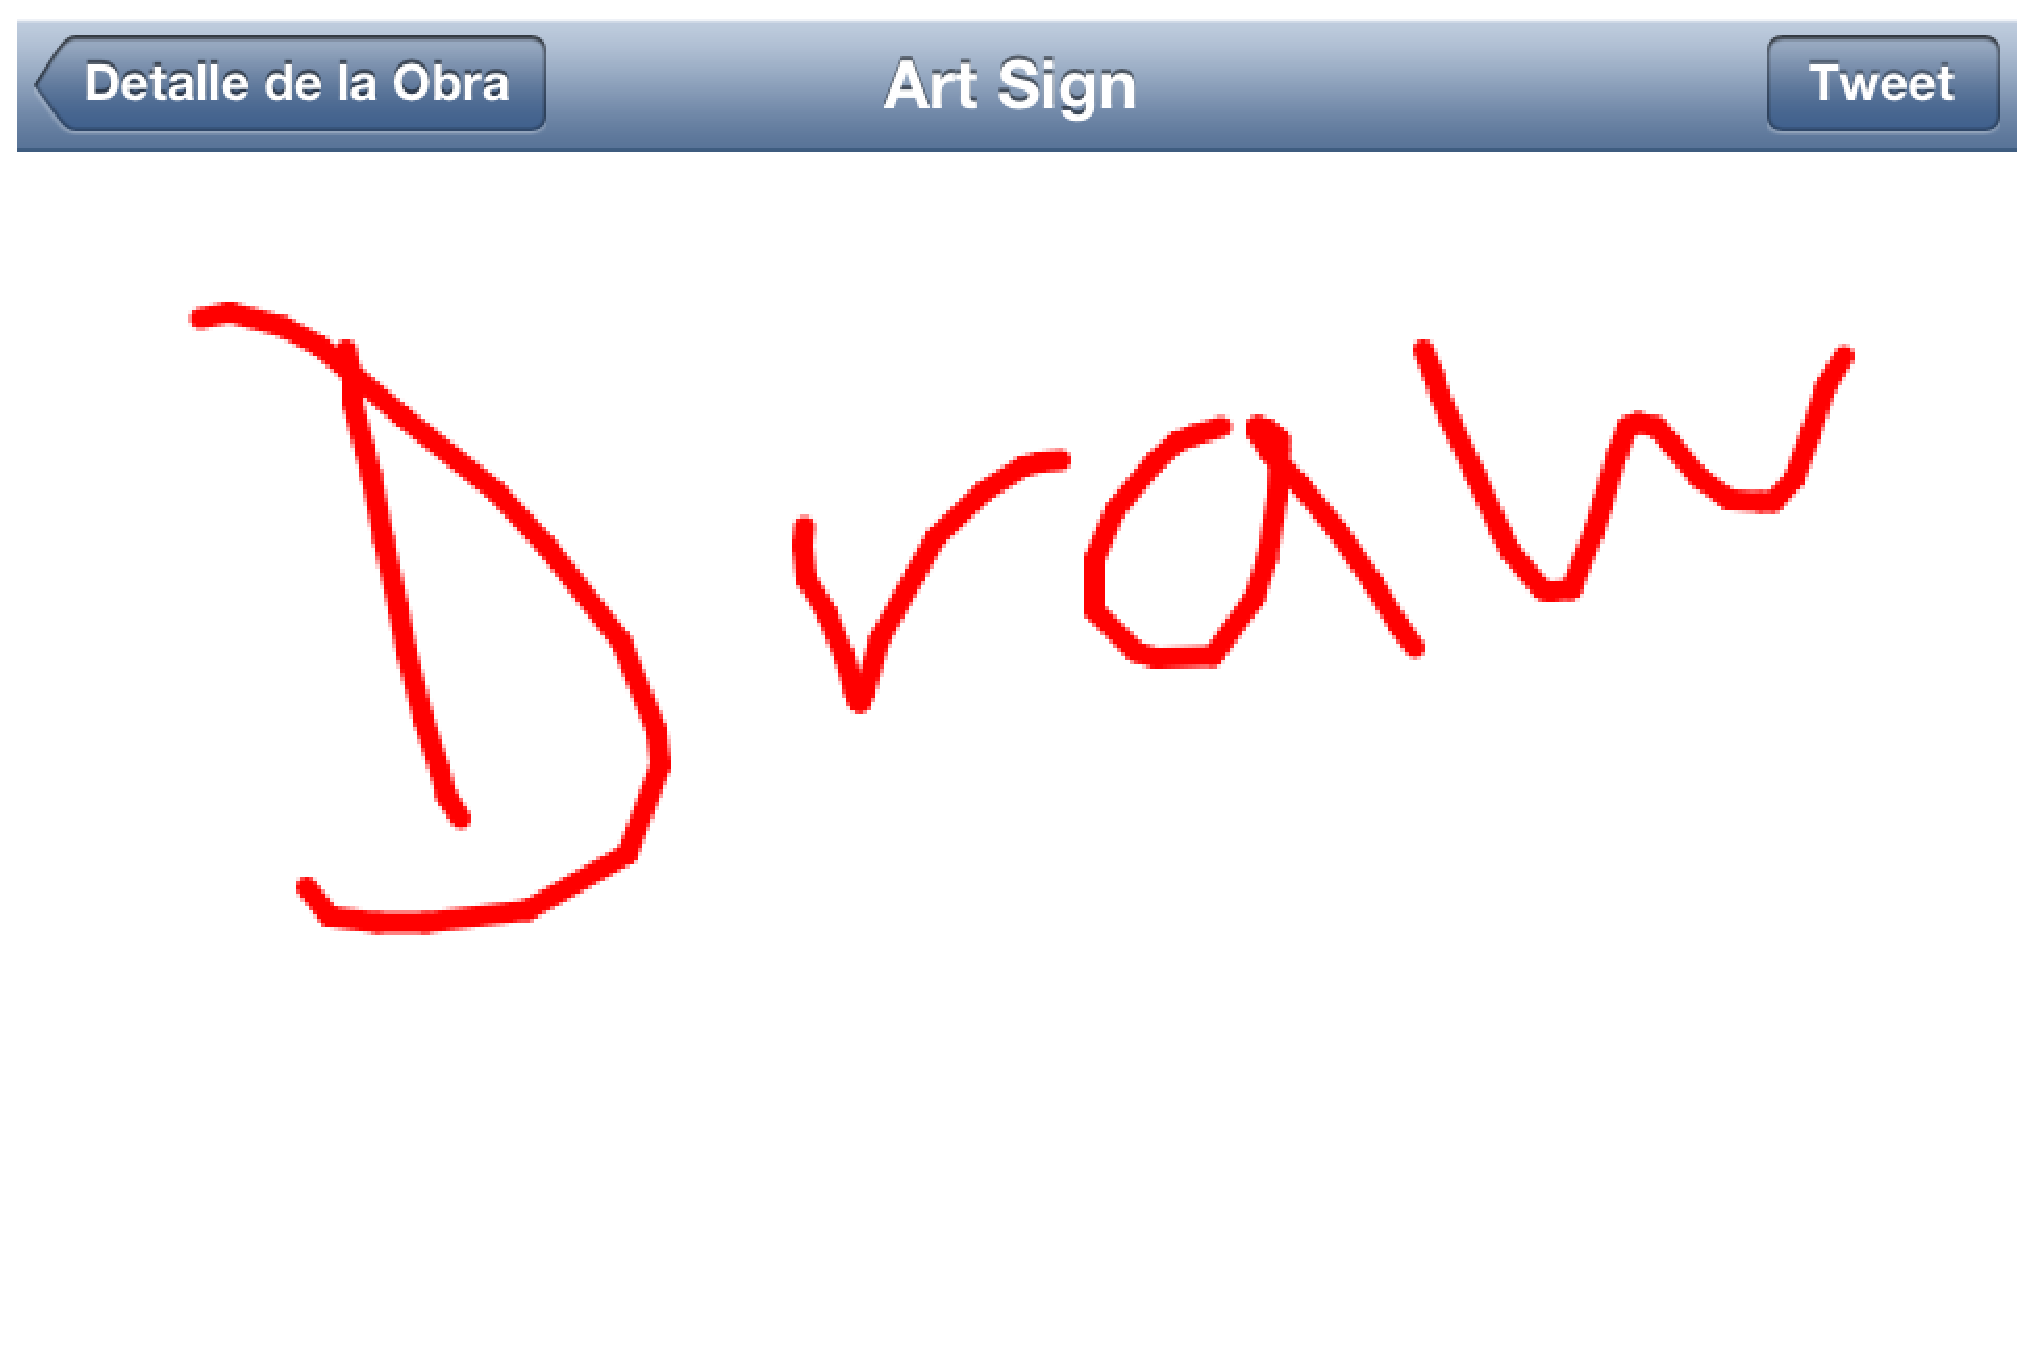
\includegraphics[scale=0.2]{figs_implementacion/Draw.eps}
\caption{Ejemplo de dibujo libre}
\label{fig: draw}
\end{figure}
Se implement� haciendo una reimplementaci�n de los siguientes tres m�todos:
\begin{verbatim}
- (void)touchesBegan:(NSSet *)touches withEvent:(UIEvent *)event;
- (void)touchesMoved:(NSSet *)touches withEvent:(UIEvent *)event;
- (void)touchesEnded:(NSSet *)touches withEvent:(UIEvent *)event;
\end{verbatim}

Cada vez que una instancia de una clase que hereda de \textit{UIViewController} detecta un toque sobre la pantalla (evento \textit{touch}), se invocan los m�todos mencionados. La secuencia de invocaciones se da al comenzar el toque en la pantalla (\textit{touchesBegan}), al desplazar el dedo sin levantarlo de la pantalla (\textit{touchesMoved}) y al finalizar el \textit{gesture} levantando el dedo de la pantalla (\textit{touchesEnded}). Un \textit{gesture} es una forma caracter�stica de tocar la pantalla. Ejemplos de \textit{gestures} existentes son: \textit{touch}, \textit{double touch}, \textit{multi touch} entre otros. Se obtienen entonces las coordenadas del punto de toque sobre la pantalla invocando el siguiente m�todo:
\begin{verbatim}
[touch locationInView:self.view]
\end{verbatim}
donde \textit{touch} es del tipo \textit{UITouch} y tiene propiedades que dependen del evento. Una vez que se tienen las coordenadas del punto de contacto en la pantalla se guarda esta posici�n y al obtener una nueva posici�n en la pantalla (luego de desplazar el dedo en \textit{touchesMoved}), se dibuja una l�nea entre el punto actual y el anterior con el m�todo siguiente:
\begin{verbatim}
[image.image drawInRect:CGRectMake(0, 0, self.view.frame.size.width,
                                       self.view.frame.size.height)];
\end{verbatim}

El m�todo \textit{drawInRect} sirve para dibujar en forma 2D sobre \textit{UIViews} y fue utilizado extensivamente en este proyecto. Finalmente en el m�todo \textit{touchesEnded} lo que se hace es dibujar una l�nea en el punto actual y s� mismo, generando un punto final al levantar el dedo de la pantalla. Otra caracter�stica interesante a mencionar respecto de la capacidad de responder a eventos \textit{touch} es el reconocimiento de \textit{gestures} que pueden ser nativos o incluso creados por el propio desarrollador. De esta manera si se quiere reconocer un \textit{double touch} por ejemplo, se puede invocar el siguiente m�todo:
\begin{verbatim}
[touch tapCount];
\end{verbatim}
que devuelve la cantidad de veces que se toc� la pantalla en un intervalo corto de tiempo. Esto fue utilizado en esta clase para borrar lo dibujado y poder comenzar a dibujar nuevamente.\\

A esta clase tambi�n se le agreg� una \textit{IBAction} que genera un \textit{tweet} con el dibujo generado por el usuario. El mismo es logrado generando una instancia de la clase \textit{TWTweetComposeViewController} y agreg�ndole un texto e imagen con los siguientes m�todos:
\begin{verbatim}
[controller setInitialText:text];
[controller addImage:img];
\end{verbatim}
donde \textit{text} e \textit{img} son el texto del \textit{tweet} y la imagen adjunta. Finalmente se presenta la \textit{view} del \textit{TWTweetComposeViewController} y una vez finalizado se vuelve a la instancia \textit{DrawSign}.
\subsection{TouchVista}
Esta clase hereda de la clase \textit{UIView} y se cre� para poder manejar eventos \textit{touch} en \textit{ViewControllers} que tienen varias \textit{subviews} y que interesa que se dispare un evento al tocar tan s�lo una de ellas en determinada �rea de la pantalla. Entonces lo que se hace en esos casos es agregar a la \textit{subview} en cuesti�n una instancia de \textit{TouchVista} en forma transparente por encima y del mismo tama\~no. De esta manera al tocar la \textit{subview} se toca en realidad la instancia de \textit{TouchVista} y se invoca el m�todo  \textit{touchesBegan}. Este m�todo simplemente configura una bandera y configura lo siguiente:
\begin{verbatim}
[super touchesBegan:touches withEvent:event];
\end{verbatim}

Lo que se hace en el c�digo anterior es invocar al m�todo \textit{touchesBegan} de la clase superior. Para el caso en que se tiene un \textit{ViewController}, con una \textit{subview} del tipo \textit{TouchVista} transparente, entonces esta l�nea invoca directamente el m�todo \textit{touchesBegan} del \textit{ViewController}. Dos de los \textit{ViewControllers} que utilizan esto son \textit{VistaViewController} y \textit{ObraCompletaViewController}.

\subsection{Realidad Aumentada en ISGL3D}
Para realizar realidad aumentada se necesita poder hacer un \textit{render} por encima de las im�genes capturadas por la c�mara del dispositivo en tiempo real. Sin embargo, cuando se crea un proyecto de ISGL3D, este permite realizar \textit{renders} pero sobre un fondo est�tico y gris (o cualquier otro color configurable). Resulta entonces necesario configurar el proyecto de manera de reemplzar al fondo antes mencionado por im�genes capturadas por la c�mara. Para lograr esto, hubo que trabajar sobre las clases \textit{Isgl3dViewController} y \textit{app0100AppDelegate}. A continuaci�n se muestran algunas modificaciones sobre estas dos clases\\
\begin{verbatim}
UIImageView* vistaImg = [[UIImageView alloc] init];

    /* Se ajusta la pantalla*/    
UIScreen *screen = [UIScreen mainScreen];
CGRect fullScreenRect = screen.bounds;   

[vistaImg setCenter:CGPointMake(fullScreenRect.size.width/2, 
fullScreenRect.size.height/2)];
[vistaImg setBounds:fullScreenRect];
    
[self.window addSubview:vistaImg];
[self.window sendSubviewToBack:vistaImg];
_viewController.videoView = vistaImg;
\end{verbatim}

Con esto se ajusta el atributo \textit{videoView} de la propiedad \textit{viewController} que pertenece a la clase \textit{app0100AppDelegate} y es instancia de la clase \textit{Isgl3dViewController}. \\

Como fue mencionado en el cap�tulo \ref{chap: hwysw}, en Xcode, si se quiere simplemente hacer una filmaci�n, sacar fotos o acceder a la galer�a de las fotos, se utiliza generalmente instancias de la clase \textit{UIImagePickerController}. Esta �ltima clase se instancia en la aplicaci�n en otras clases, como ser \textit{ImagenServerViewController}. Si lo que se desea es acceder a los p�xeles de las im�genes capturadas, para luego poder procesarlos en tiempo real, entonces la forma m�s indicada es usando el conocido \textit{framework} \textit{AVFoundation}. En la clase \textit{Isgl3dViewController}, en el m�todo \textit{viewDidLoad} est� toda la configuraci�n necesaria para la utilizaci�n de \textit{AVFoundation}. A continuaci�n se muestra el c�digo con sus comentarios sobre esta configuraci�n.\\
\begin{verbatim}
/*Creamos y seteamos la captureSession*/
    self.session = [[AVCaptureSession alloc] init];
    self.session.sessionPreset = AVCaptureSessionPresetMedium;
    
    /*Creamos al videoDevice*/
    self.videoDevice = [AVCaptureDevice defaultDeviceWithMediaType:AVMediaTypeVideo];
    
    /*Creamos al videoInput*/
    self.videoInput  = [AVCaptureDeviceInput deviceInputWithDevice:
    self.videoDevice error:nil];
    
    /*Creamos y seteamos al frameOutpt*/
    self.frameOutput = [[AVCaptureVideoDataOutput alloc] init];
    
    self.frameOutput.videoSettings = [NSDictionary dictionaryWithObject:
    [NSNumber numberWithInt:kCVPixelFormatType_32BGRA] forKey:(id)
     kCVPixelBufferPixelFormatTypeKey];
    
    /*Ahora conectamos todos los objetos*/
    /*Primero le agregamos a la sesion el videoInput y el videoOutput*/
    
    [self.session addInput: self.videoInput];
    [self.session addOutput: self.frameOutput];
\end{verbatim}

Como se ve, es necesario crear una sesi�n de captura, luego un dispositivo de captura y una salida de los datos y agregarlos a la sesi�n. Tambi�n se puede configurar el tipo de captura de la c�mara (tiene que ser soportado por el \textit{hardware}, sino se genera un error en este punto). \\
Otra cosa importante que se hace en la clase \textit{Isgl3dViewController} es la configuraci�n del \textit{multithreading}. A continuaci�n se muestra el c�digo que logra esto.
\begin{verbatim}
    dispatch_queue_t processQueue = dispatch_queue_create("procesador", NULL);
    [self.frameOutput setSampleBufferDelegate:self queue:processQueue];
    dispatch_release(processQueue);
\end{verbatim}

Con esto lo que se hace es hacer una instancia de una \textit{Queue}, que representa una cola de procesamiento. De esta manera se puede hacer que ciertas tareas se alojen en esa instancia de cola, que l�gicamente es otra distinta que la cola de procesamiento principal (\textit{mainQueue}). Esto mismo es lo que se hace en la segunda l�nea del c�digo anterior, diciendo que el \textit{Delegate} de los datos de salida (\textit{frameOutput}) es la propia clase y que ese \textit{Delegate} se ejecute en la \textit{Queue} que se instanci� en la l�nea anterior. De esta manera todo lo que sea invocado por el \textit{Delegate} en forma peri�dica ser� enviado a una cola distinta de la principal, pudiendo tener entonces, una cola de procesamiento separada de la cola de interfaz de usuario. Esto es algo ampliamente utilizado y es una recomendaci�n de la documentaci�n de iOS, pues se basa en los conceptos de tener la mayor atenci�n posible a la interfaz de usuario, impidiendo en lo posible dejar al usuario esperando por alg�n eventual procesamiento que se est� llevando a cabo.\\
Finalmente se da comienzo a la sesi�n:\\
\begin{verbatim}
[self.session startRunning];
\end{verbatim}
Como la clase \textit{Isgl3dViewController} implementa el protocolo 			textit{AVCaptureVideoDataOutputSampleBufferDelegate}, una vez que comienza la sesi�n, se invoca cuadro a cuadro el siguiente m�todo:\\
\begin{verbatim}
-(void) captureOutput:(AVCaptureOutput *)captureOutput didOutputSampleBuffer
:(CMSampleBufferRef)sampleBuffer fromConnection:(AVCaptureConnection *)connection;
\end{verbatim}
donde \textit{sampleBuffer} es una referencia al \textit{buffer} que contiene los p�xeles de la c�mara en ese momento. As� entonces, se accede a los p�xeles y se invoca dentro del \textit{captureOutput} peri�dicamente al m�todo \textit{procesamiento}, encargado de procesar la imagen recibida por la c�mara.
\section{El QR en la aplicaci�n}
\label{sec: QR}
Para el prototipo de aplicaci�n se opt� por tener un identificador QR para cada uno de los tres artistas elegidos del Museo Nacional de Artes Visuales (MNAV). De esta manera, para el caso del recorrido del museo de forma autom�tica, es posible determinar la posici�n del usuario utilizando im�genes QR debidamente ubicadas en cada zona. Esto sirve como localizaci�n y tambi�n sirve para lograr que el paso siguiente, que es la identificaci�n de la obra que el usuario tiene enfrente, sea mediante una b�squeda en una base de datos discriminada por autor como se explic� en la secci�n \ref{fig: imagenServer}. Es decir, si el usuario no escanea el QR la b�squeda de la obra a identificar se har� en una base de datos global del museo, pero en el caso que el usuario s� decida escanear el QR, entonces se cuenta con la posibilidad de realizar la b�squeda en una base de datos reducida y por lo tanto m\'as veloz. \\




\section{Servidor}
Si bien el desarrollo de la aplicaci�n busca lograr un prototipo y no una aplicaci�n comercial, por lo que la cantidad de im�genes y datos en general es peque\~na y por lo tanto puede ser almacenada dentro de la aplicaci�n, por prolijidad y escalabilidad resulta imprescindible contar con un servidor. Es necesario un servidor que guarde la toda la informaci�n y a la vez realice algo de procesamiento, siempre y cuando este no deba hacerse en tiempo real. Se decidi� entonces, almacenar toda aquella informaci�n relevante en cuanto a registro de obras (im�genes, t�tulos, autores y descripciones), audiogu�as, videos, modelos y animaciones utilizadas para la realidad aumentada en un servidor que hubo que implementar. El servidor debe estar hubicado dentro del museo y se debe poder interactuar con �l por medio de la LAN ($54$ Mbps). Si bien es cierto que el servidor podr�a perfectamente ser remoto, con acceso por medio de internet, su desempe\~no a nivel de tiempos bajar�a notoriamente.

\subsection{Creando el servidor}
Para la creaci�n del servidor se busc� primeramente la alternativa de hacerlo sobre una m�quina con sistema operativo con n�cleo Linux, distribuci�n Ubuntu, ya que se crey� ser�a m�s sencillo. Luego de realizada esta tarea, se estudi� la posibilidad de tener el servidor corriendo sobre una plataforma Mac OS X y de manera sorpresiva, en este segundo caso, el objetivo se logr� de forma mucho m�s sencilla. A continuaci�n se explica paso por paso como se implementaron los servidores en uno y otro sistema operativo.

\subsubsection{Servidor LAMP}
Se le llama LAMP a la combinaci�n de todas las herramientas necesarias para lograr un servidor web: Linux (Sistema Operativo), Apache (Servidor Web), MySQL (Gestor de base de datos) y PHP/Perl/Python (lenguaje de programaci�n del lado del servidor). Se comenz� entonces por instalar un servidor web Apache, que tiene como principales ventajas el hecho de ser multiplataforma, gratis y de c�digo abierto. La descarga y la instalaci�n son inmediatas, se abre un terminar y se escribe:
\begin{verbatim}
sudo apt-get install apache2
\end{verbatim}
Una vez finalizada la instalaci�n de este congjunto de paquetes ya se cuenta con el servidor y mediante los siguientes comandos, uno puede dar inicio y fin al mismo:
\begin{verbatim}
sudo /etc/init.d/apache2 start
sudo /etc/init.d/apache2 stop
\end{verbatim}
Luego de tener instalado Apache, se procede a instalar php:
\begin{verbatim}
sudo apt-get install php5
\end{verbatim}
%fuente http://www.guia-ubuntu.org/index.php?title=Servidor_web
Para este proyecto en particular, no fue necesario instalar MySQL.

\subsubsection{Servidor en Mac OS X}
A diferencia de otros sistemas operativos, Mac OS X cuenta por defecto con Apache y Php, no as� con MySQL. Para tener un servidor entonces, s�lo resta activarlos y si adem�s se quiere contar con MySQL, es necesario instalarlo. La activaci�n del servidor es un proceso muy simple, del cual existe bastante material disponible en internet.\\

Una vez instalado el servidor en cualquiera de ambos sistemas operativos, se puede corroborar su correcto funcionamiento abriendo cualquier navegador web y digitando la direcci�n IP de la m�quina en la que se instal� el servidor (si se est� en ella misma, se puede digitar la direcci�n del bucle local). Se deber� ver la p�gina que por defecto muestra el servidor, la de la figura \ref{fig: implementacion_4}.

\begin{figure}[h!]
\centering
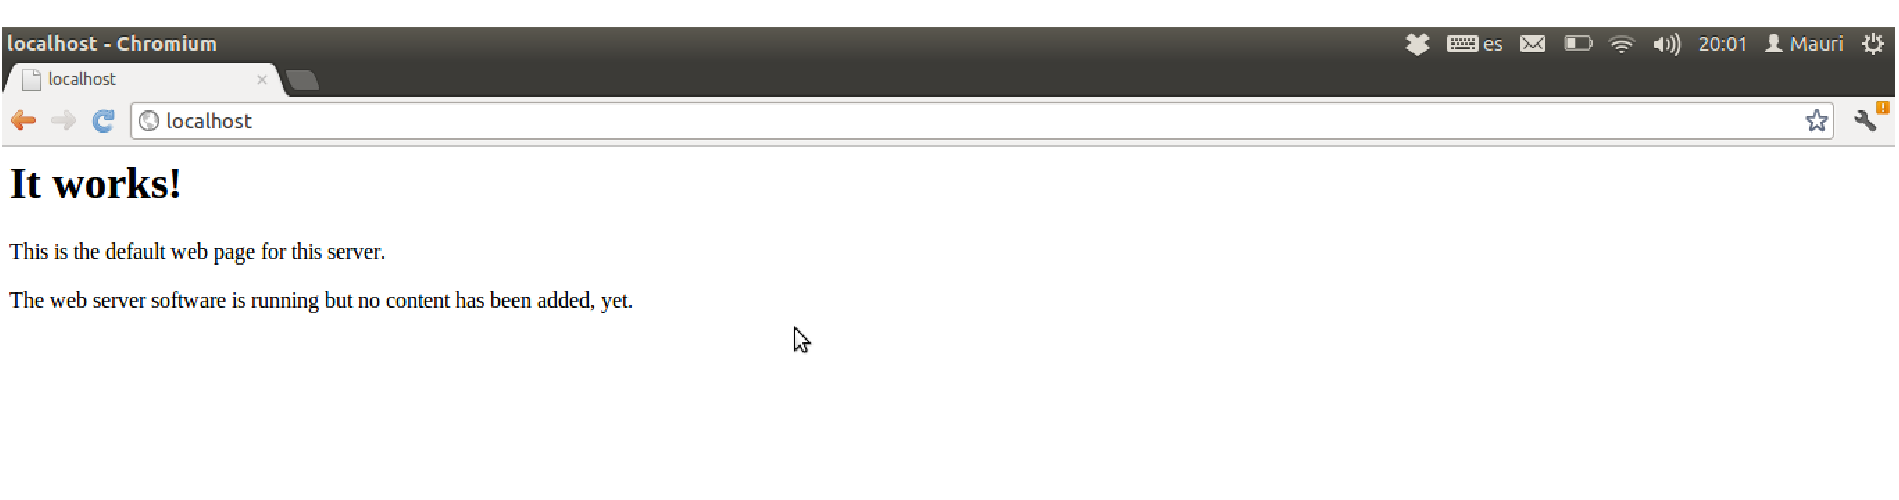
\includegraphics[scale=0.3]{figs_implementacion/Itworks2.png}
\caption{P�gina por defecto del servidor Apache.}
\label{fig: implementacion_4}
\end{figure}

\subsubsection{Aspectos a mejorar del Servidor}
Como se mencion� el servidor se implement� sin MySQL y tampoco con ning�n otro gestor de base de datos, lo que hace que cualquier modificaci�n sobre la informaci�n de los cuadros, ya sea en cuanto a im�genes, descripciones, audiogu�as o cualquier informaci�n que se quiera modificar dentro del servidor hace que quien administre el mismo tenga la necesidad de comprender en cierta medida c�mo est� implementado y tener cierto dominio t�cnico. Para el caso de aplicar esto en un museo y pensando que quienes administren la informaci�n de los cuadros sea gente encargada del museo no especializada en aspectos de software, es deseable que la interfaz de gesti�n del servidor tenga un entorno m�s amigable. Esto es algo que se podr�a mejorar para un futuro en caso de querer continuar trabajando con el presente proyecto para darle m�s completitud y usabilidad.

%--------------------------------------------------------------------------------------------------- |SIFT| -------------------------------------------------------------------------------------
\section{SIFT}
\label{sec: sift}

SIFT fue utilizado en el presente proyecto para el reconocimiento de las obras contempladas por los usuarios, cuando estos deciden realizar el recorrido interactivo del museo de forma autom\'atica. El algoritmo corre en el servidor y el c\'odigo utilizado es una adaptaci\'on propia de la implementaci\'on en C que est� en la librer\'ia VL-Feat. VL-Feat es una librer\'ia gratis y en c\'odigo abierto que implementa algoritmos populares de visi\'on artificial que puede ser descargada de su p\'agina web oficial \cite{vlfeat12}. \\

% ------------------------------------------------------------------------------------------------------------------------------------------

Se tiene entonces, para cada obra en cuesti\'on, una lista de 128 descriptores invariantes a factores de escala, traslaci\'on, rotaci\'on y parcialmente invariantes a cambios de iluminaci\'on y afinidades; almacenada en el servidor. Cuando el usuario se encuentra frente a una obra determinada, este le toma una fotograf\'ia y esta es subida al servidor, en donde es procesada con SIFT y luego sus descriptores son comparados contra todos los descriptores de la base de datos, o al menos los correspondientes a la regi\'on del museo en donde el usuario se encuentra. La obra con m\'as descriptores en com\'un con la imagen en cuesti\'on ser\'a la que el usuario contempla.\\



% ------------------------------------------------------------------------------------- |COMENTARIOS SOBRE LA IMPLEMENTACI�N| ---------------------------------------------------------------------------
\section{Comentarios finales sobre la implementaci�n}
Hasta el momento se mencionaron una cantidad de herramientas m�s que interesantes, que reunidas logran un recorrido interactivo para uno o m�s museos. Sin embargo, no se expusieron cu�les son las aplicaciones puntuales de realidad aumentada que se dijo se iba a hacer sobre las obras. Por otra parte, aunque dejando afuera aspectos est�ticos y art�sticos, en el cap�tulo \ref{chap: casoUso} se mostr� como se resolvieron los aspectos t�cnicos necesarios para llevar a cabo una aplicaci�n final real de realidad aumentada. As� entonces el generar un \textit{render} de un perro junto a un sill�n (caso de uso ``modelos''), que claramente puede llegar a ser de muy poco inter�s para un museo, resuelve el mismo problema que si se quisiera generar un \textit{render} con el modelo de Jos� Artigas. Asimismo ser capaz de responder frente a al toque en la pantalla del modelo de un cubo y as� entonces actuar en consecuencia (caso de uso ``interactivo''), resuelve el mismo problema que animar al modelo de Jos� Artigas si este es tocado. Lo que se tiene en este caso (y efectivamente se logr�), es una escultura digital e interactiva de Artigas, que s�lo puede visualizarse a trav�s de un \textit{iPad}. Ver figura \ref{fig:artigases}.\\ 

\begin{figure}[h!]
\centering
$
\begin{array}{cc}
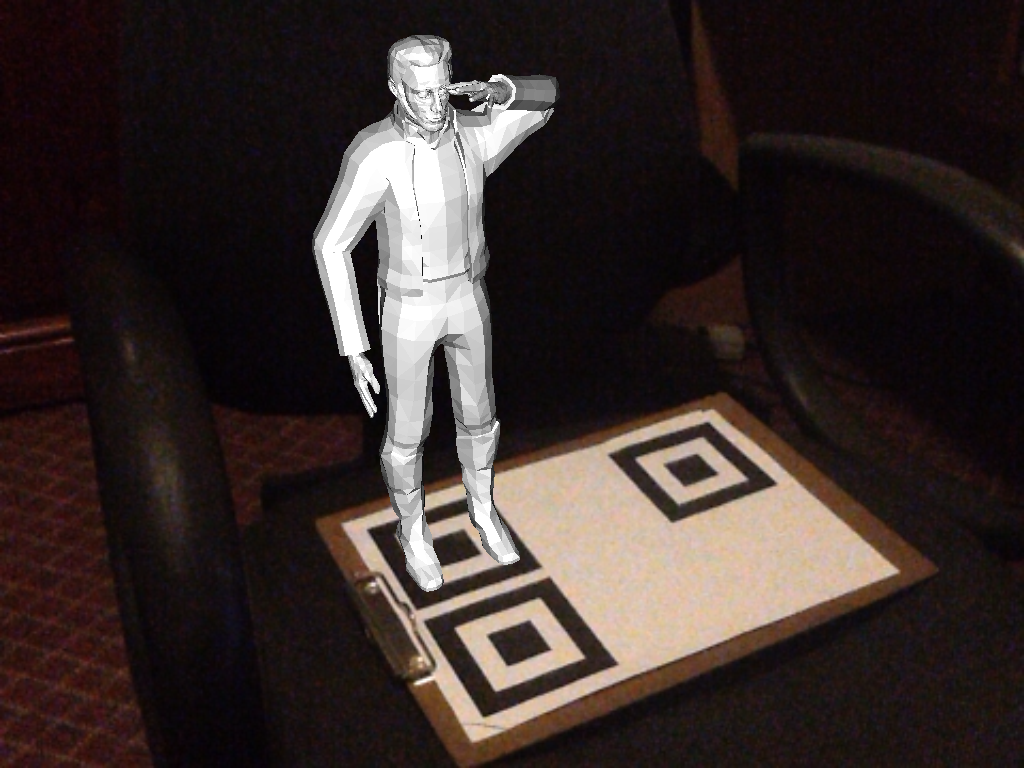
\includegraphics[scale=0.2]{figs_implementacion/artigas_1.png} & 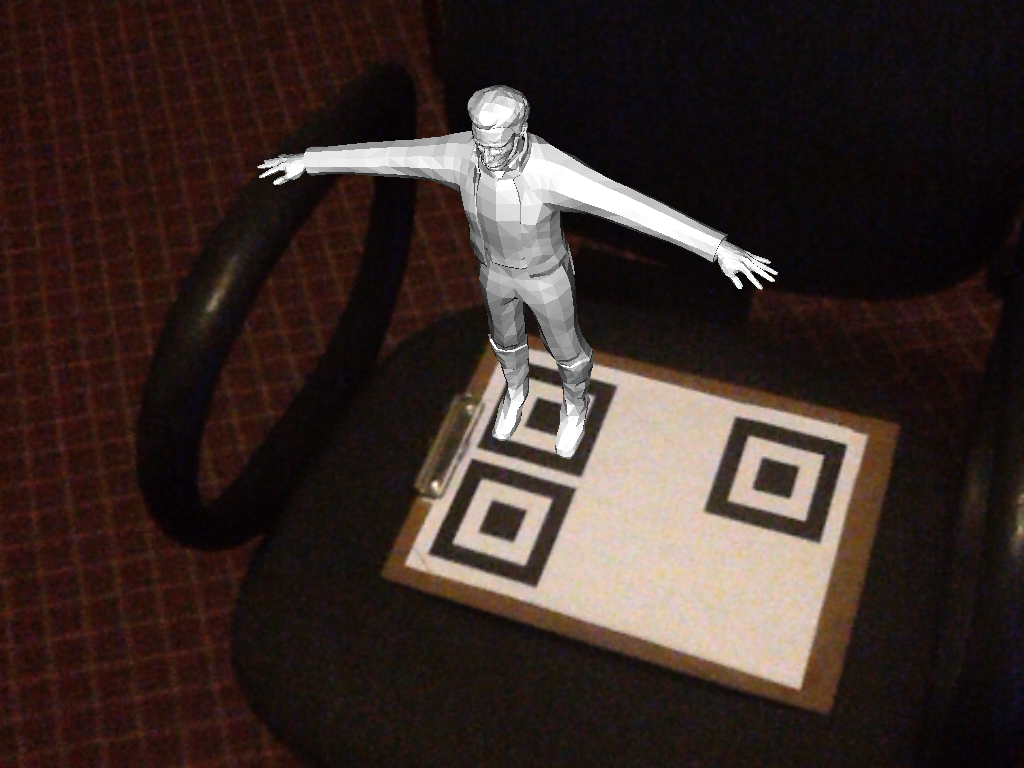
\includegraphics[scale=0.2]{figs_implementacion/artigas_2.png} \\
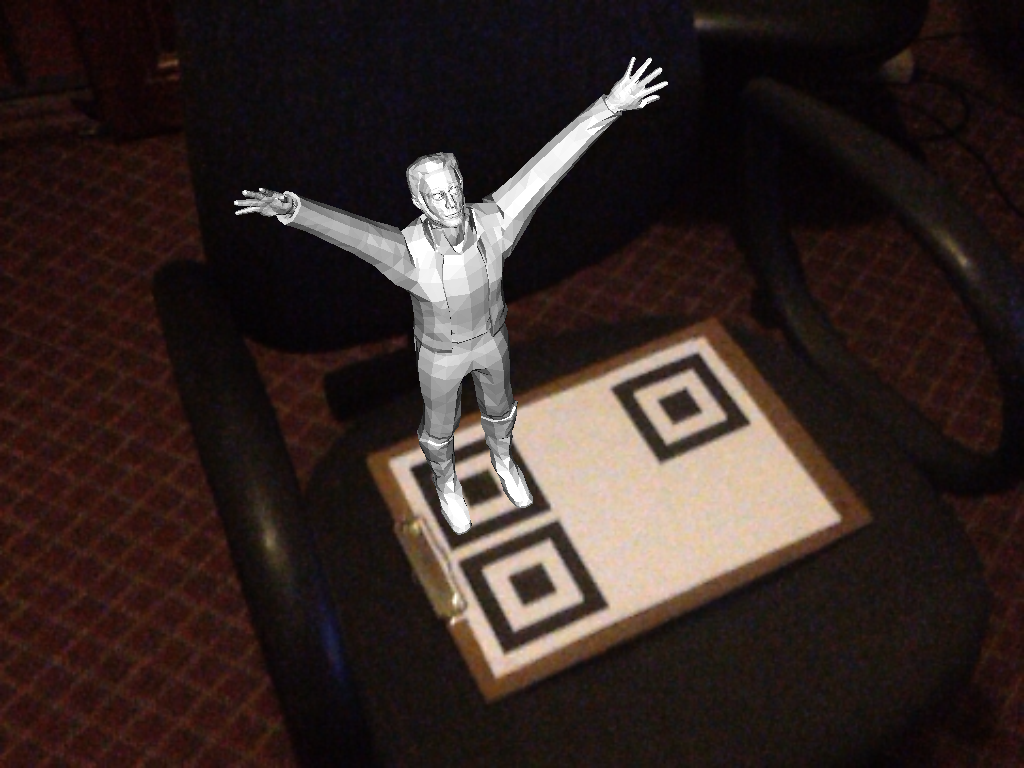
\includegraphics[scale=0.2]{figs_implementacion/artigas_3.png} & 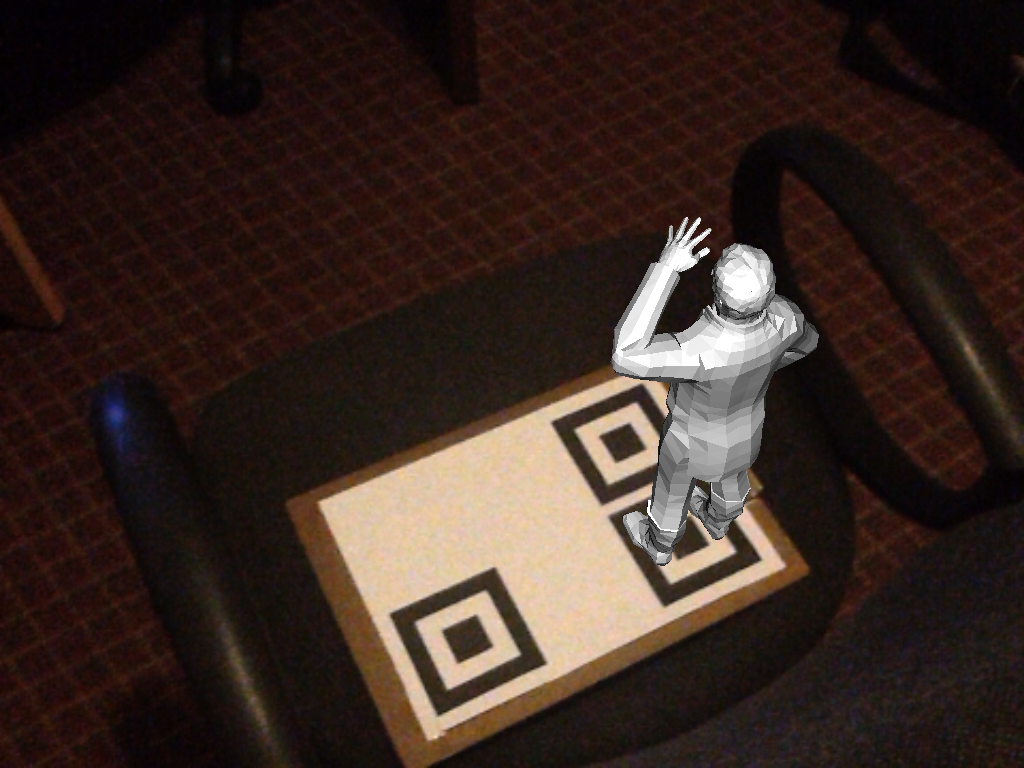
\includegraphics[scale=0.2]{figs_implementacion/artigas_4.png}
\end{array}
$
\caption{Escultura digital e interactiva de Artigas vista desde �ngulos distintos y en posiciones distintas.}
\label{fig:artigases}
\end{figure}


Lo mismo sucede con el caso de uso ``video'', que proyecta un video sobre el marcador, que puede facilmente adaptarse para proyectar un video de inter�s sobre una obra, parte de ella o incluso un mapa con informaci�n del museo o cualquier otra cosa. As� entonces logrando una audiogu�a interactiva, donde el usuario puede, mientras se le habla de la obra, ver fotos y videos realacionados a la misma. A la fecha se est� buscando aplicar, dentro de lo posible, los desaf�os t�cnicos resueltos en cada uno de los casos de uso mencionados en el cap�tulo \ref{chap: casoUso} a diferentes implementaciones que puedan llegar a resultar atractivas para uno o varios museos. Las opciones son much�simas y se cree que este proyecto deja una puerta abierta a seguir explorando ideas innovadoras.\\


% Ejemplo de como hacer una cita:
\cite{Daniel03simultaneouspose}.



\bibliographystyle{unsrt}   
\bibliography{encuadro}  
\end{document}